\chapter{Сферическое движение твердого тела. Уравнения движения. Углы Эйлера.
Определение скорости произвольной точки твердого тела. Кинематические
уравнения Эйлера. Уравнение мгновенной оси вращения.}
Движение тела, имеющую одну неподвижную точку, называют сферическим движением
или вращением тела вокруг неподвижной точки. При таком движении траектории точек
тела лежат на сферах.

\begin{table}[h!]
    \vspace*{-1em}
    \begin{tabular}{C{.4}m{.55\textwidth}}
        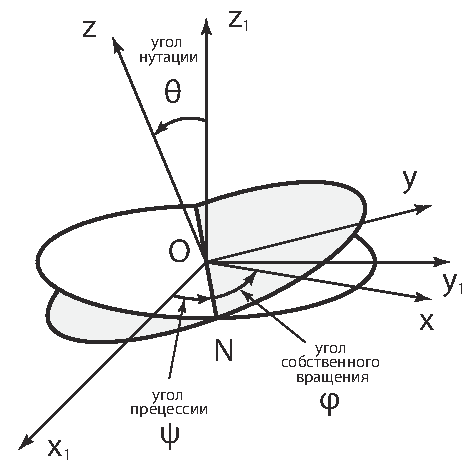
\includegraphics[width=.4\textwidth]{32_01} &
        Тело с одной закрепленной точкой имеет три вращательных степени свободы,
        поэтому естественно выбрать в качестве координат углы. В теоретической
        механике, как правило, в их роли выступают углы Эйлера. Вводятся они
        следующим образом:

        выберем неподвижную систему координат \( Ox_1y_1z_1 \), а с телом жестко
        свяжем систему координат \( Oxyz \). Плоскости \( Oxy \) и \( Ox_1y_1 \)
        пересекаются по прямой \( ON \), которая называется линией узлов.

        Угол между линией узлов и неподвижной осью \( Ox_1 \) называется углом
        прецессии \( \psi \).
    \end{tabular}
    \vspace*{-1em}
\end{table}
Угол между осями \( Oz_1 \) и \( Oz \) называется углом нутации \( \theta \).

И, наконец,
угол между линией узлов и подвижной осью \( Ox \) называется углом собственного
вращения \( \phi \).

Определим теперь скорость произвольной точки тела, к примеру точки \( M \). Её
положение определяется радиус-вектором \( \vec{r} = x\vec{e}_x + y\vec{e}_y +
z\vec{e}_z \). В системе координат, жестко связанной с телом \( x \), \( y \) и
\( z \) -- постоянные, поэтому
\( \ds \vec{v} = \der{\vec{r}}{t} = x\der{\vec{e}_x}{t} + y\der{\vec{e}_y}{t} +
z\der{\vec{e}_z}{t} \).

Так как базис \( (\vec{e}_x, \vec{e}_y, \vec{e}_z) \) -- ортонормированный, то
\[
    \left\{ \begin{array}{l}
        \ds\der{\vec{e}_x}{t} = \vec{\omega}\times\vec{e}_x, \\[.6em]
        \ds\der{\vec{e}_y}{t} = \vec{\omega}\times\vec{e}_y, \\[.6em]
        \ds\der{\vec{e}_z}{t} = \vec{\omega}\times\vec{e}_z,
    \end{array} \right| \Rightarrow
    \vec{v} = \vec{\omega}\times(x\vec{e}_x + y\vec{e}_y + z\vec{e}_z) =
    \vec{\omega}\times\vec{r},
\]
где \( \vec{\omega} \) -- вектор мгновенной угловой скорости.

Геометрическое место точек, скорость которых равна 0 называется мгновенной осью
вращения: \( \vec{\omega}\times\vec{r} = 0 \), откуда получаем уравнение
мгновенной оси вращения: \( \ds \frac{x}{\omega_x} = \frac{y}{\omega_y} =
\frac{z}{\omega_z} \).

Теперь получим кинематические уравнения Эйлера:
\[
    \vec{\omega} = \omega_\psi\vec{e}_{z_1} + \omega_\theta\vec{e}_N +
    \omega_\phi\vec{e}_z = \omega_x\vec{e}_x + \omega_y\vec{e}_y +
    \omega_z\vec{e}_z.
\]

Помножим скалярно на орты \( \vec{e}_x \), \( \vec{e}_y \) и \( \vec{e}_z \),
получим выражения для \( \omega_x \), \( \omega_y \) и \( \omega_z \) через
производные по времени от углов Эйлера:
\[
    \left\{ \begin{array}{l}
        \omega_x = \omega_\psi\vec{e}_{z_1}\cdot\vec{e}_x +
        \omega_\theta\vec{e}_N\cdot\vec{e}_x +\omega_\phi\vec{e}_z\cdot\vec{e}_x
        = \dot{\psi}\sin\theta\sin\phi + \dot{\theta}\cos\phi, \\
        \omega_y = \omega_\psi\vec{e}_{z_1}\cdot\vec{e}_y +
        \omega_\theta\vec{e}_N\cdot\vec{e}_y +\omega_\phi\vec{e}_z\cdot\vec{e}_y
        = \dot{\psi}\sin\theta\cos\phi - \dot{\theta}\sin\phi, \\
        \omega_z = \omega_\psi\vec{e}_{z_1}\cdot\vec{e}_z +
        \omega_\theta\vec{e}_N\cdot\vec{e}_z +\omega_\phi\vec{e}_z\cdot\vec{e}_z
        = \dot{\psi}\cos\theta + \dot\phi.
    \end{array} \right.
\]

Это и есть кинематические уравнения Эйлера.
\newpage
